\begin{frame}
\tableofcontents
\end{frame}

\hypertarget{introduction}{%
\section{Introduction}\label{introduction}}

\begin{frame}{Contexte}
\protect\hypertarget{contexte}{}
\begin{itemize}
\tightlist
\item
  RTE : gestion du réseau haute tension français
\item
  2,5\% de la consommation perdue : 500 M€
\item
  Objectif : modèle de prédiction de pertes
\end{itemize}
\end{frame}

\begin{frame}{Problématique}
\protect\hypertarget{probluxe9matique}{}
\begin{itemize}
\tightlist
\item
  35 variables explicatives
\item
  Prédiction à long terme (1 an)
\end{itemize}
\end{frame}

\begin{frame}{Ressources}
\protect\hypertarget{ressources}{}
\begin{itemize}
\tightlist
\item
  Base de données : 35 variables et pertes horaires
\item
  Rapport de stage sur la prédiction de pertes
\end{itemize}
\end{frame}

\begin{frame}{Objectif}
\protect\hypertarget{objectif}{}
\begin{itemize}
\tightlist
\item
  Identifier les variables significatives
\item
  Identifier et paramétrer un algorithme de prédiction efficace
\end{itemize}
\end{frame}

\hypertarget{ruxe9cupuxe9ration-des-donnuxe9es}{%
\section{Récupération des
données}\label{ruxe9cupuxe9ration-des-donnuxe9es}}

\begin{frame}{Réception}
\protect\hypertarget{ruxe9ception}{}
\begin{itemize}
\tightlist
\item
  Activité du réseau (consommation, production, énergie) : eco2mix
\item
  Pertes relevées : portail client RTE
\end{itemize}
\end{frame}

\begin{frame}{Visualisation}
\protect\hypertarget{visualisation}{}
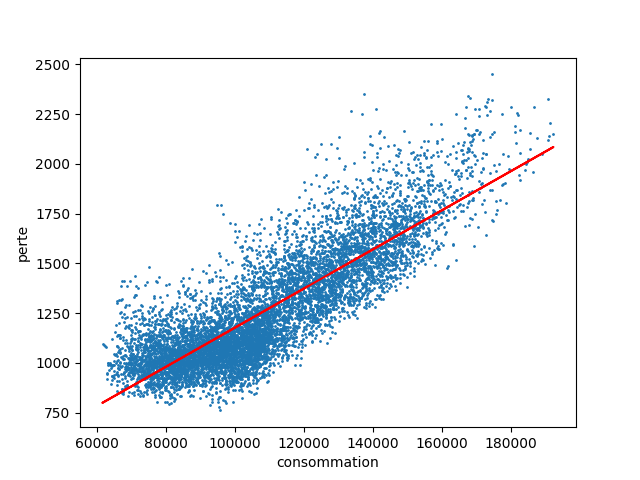
\includegraphics[scale=.5]{figures/scatter_consommation_2018.png}
\end{frame}

\begin{frame}{Description}
\protect\hypertarget{description}{}
\begin{itemize}
\tightlist
\item
  date/heure : représentatif de l'activité et du climat
\item
  consommation, prévisions : charge et imprévus
\item
  production : régimes d'activation et de charge du réseau
\item
  échanges : charge supplémentaire sur des points individuels
\end{itemize}
\end{frame}

\begin{frame}[fragile]{Traitement des fichiers}
\protect\hypertarget{traitement-des-fichiers}{}
\begin{itemize}
\tightlist
\item
  encodage utf-8, comma separated values
\item
  colonnes en \texttt{snake\_case}
\item
  dates/heures numériques
\end{itemize}

pertes au même format que les données de
consommation/production/échanges :

\begin{itemize}
\tightlist
\item
  élimination des lignes parasites (commentaires)
\item
  un fichier par an
\item
  une ligne par heure (colonnes jour/mois pour accès facile en
  observation)
\end{itemize}
\end{frame}

\hypertarget{algorithmes-de-pruxe9diction}{%
\section{Algorithmes de prédiction}\label{algorithmes-de-pruxe9diction}}

\begin{frame}{Régression linéaire}
\protect\hypertarget{ruxe9gression-linuxe9aire}{}
Dépendance linéaire à déterminer : \begin{equation}
f(x, \epsilon) = \beta_0 + \sum_{j=1}^p \beta_jx^j + \epsilon
\end{equation}

Résultats selon le pré-traitement des données :

\begin{longtable}[]{@{}ll@{}}
\toprule
\textbf{traitement} & \textbf{\(R^2\)}\tabularnewline
\midrule
\endhead
normalisées & 0.80\tabularnewline
standardisées & 0.83\tabularnewline
orthogonalisées & -1.9\tabularnewline
\bottomrule
\end{longtable}
\end{frame}

\begin{frame}{Régression linéaire}
\protect\hypertarget{ruxe9gression-linuxe9aire-1}{}
De bons résultats en standardisant les données :
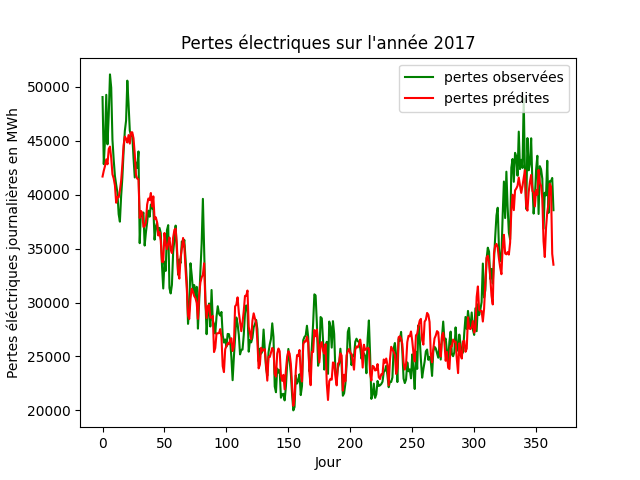
\includegraphics[scale=.5]{figures/2017_st.png}
\end{frame}

\begin{frame}{Machine à noyaux}
\protect\hypertarget{machine-uxe0-noyaux}{}
Coefficient de détermination selon le prétraitement :

\begin{longtable}[]{@{}ll@{}}
\toprule
\textbf{traitement} & \textbf{\(R^2\)}\tabularnewline
\midrule
\endhead
normalisées & 0.63\tabularnewline
standardisées & 0.61\tabularnewline
orthogonalisées & -0.17\tabularnewline
\bottomrule
\end{longtable}
\end{frame}

\begin{frame}{Machine à noyau}
\protect\hypertarget{machine-uxe0-noyau}{}
Résultats avec la machine à noyau, données standardisées :
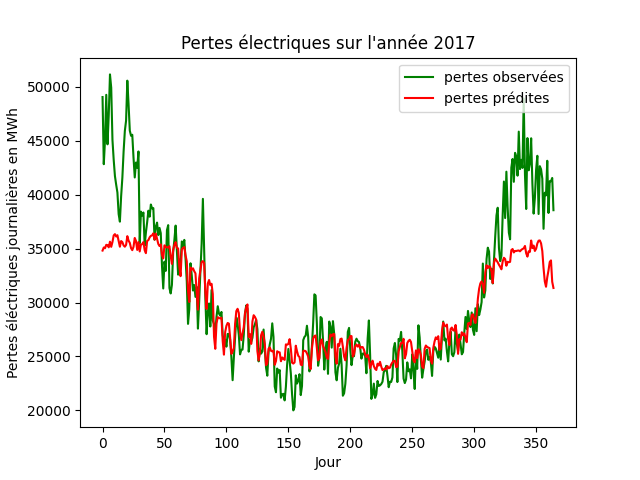
\includegraphics[scale=.5]{figures/svr_2017.png}
\end{frame}

\begin{frame}{Réseau de neurones}
\protect\hypertarget{ruxe9seau-de-neurones}{}
\begin{itemize}
\tightlist
\item
  utilisation de Tensorflow
\item
  structure du réseau :
\end{itemize}

\begin{longtable}[]{@{}ll@{}}
\toprule
\textbf{neurones} & \textbf{activation}\tabularnewline
\midrule
\endhead
35 & (entrée)\tabularnewline
400 & sigmoïde\tabularnewline
400 & sigmoïde\tabularnewline
100 & ReLU\tabularnewline
1 & linéaire (sortie)\tabularnewline
\bottomrule
\end{longtable}
\end{frame}

\hypertarget{suxe9lection-de-variables}{%
\section{Sélection de variables}\label{suxe9lection-de-variables}}

\begin{frame}{Élimination des doublons}
\protect\hypertarget{uxe9limination-des-doublons}{}
Corrélation de Pearson :
\(\rho(X,Y) = \frac{cov(X, Y)}{\sigma_X\sigma_Y}\)
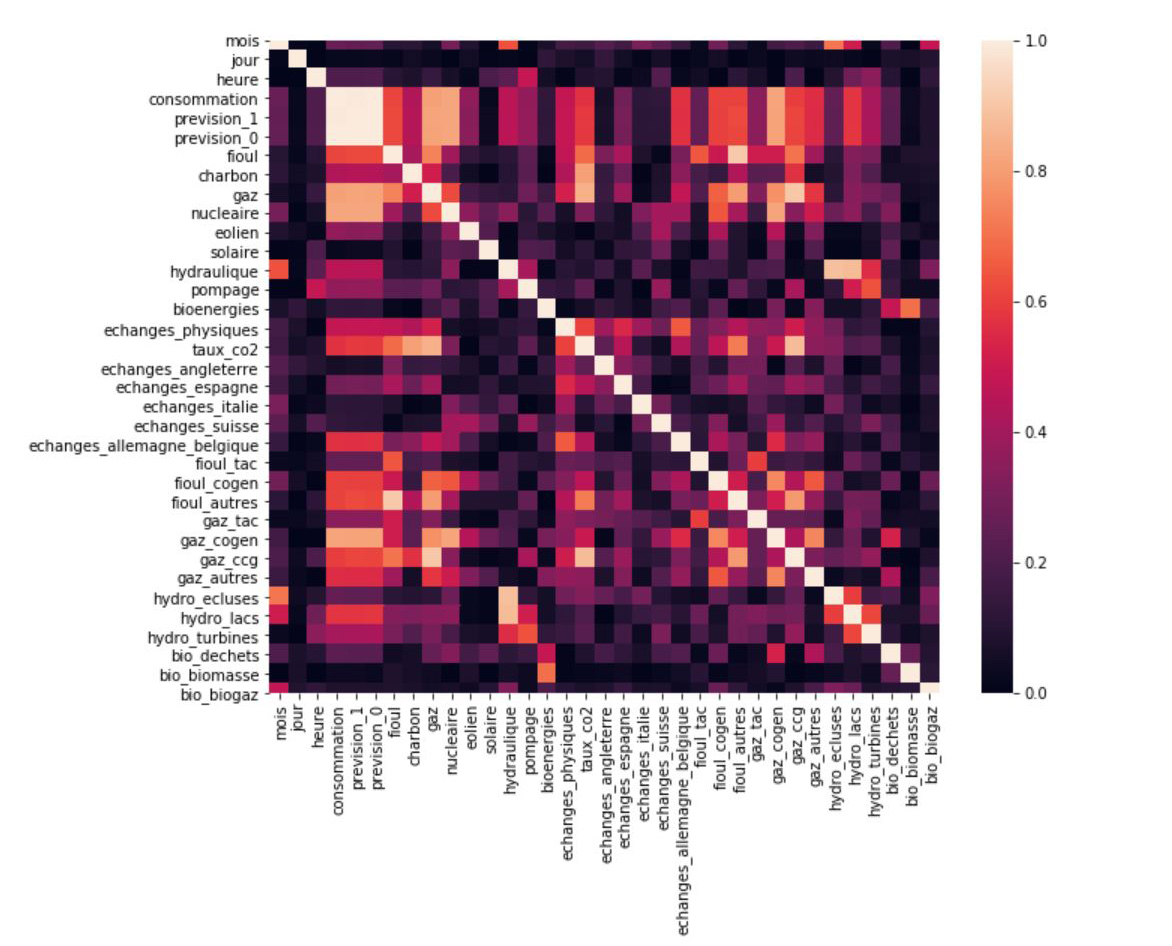
\includegraphics[scale=.4]{figures/heatmap.jpg}
\end{frame}

\begin{frame}[fragile]{Élimination des doublons}
\protect\hypertarget{uxe9limination-des-doublons-1}{}
Coefficient de détermination selon le seuil d'élimination :
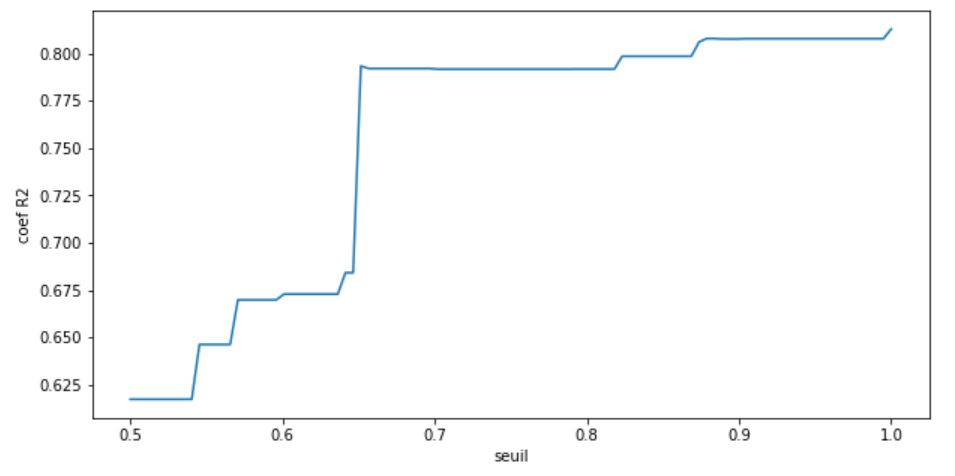
\includegraphics[scale=.5]{figures/doublons.JPG}

seuil à \(0.8 > 0.65\), supprimant \texttt{consommation},
\texttt{prevision\_0}, \texttt{fioul}, \texttt{gaz},
\texttt{hydraulique}, \texttt{hydro\_lacs}, \texttt{taux\_co2}, 1.4\% de
perte

\texttt{prevision\_1} moins bruitée que \texttt{consommation}
\end{frame}

\begin{frame}{Élimination des doublons}
\protect\hypertarget{uxe9limination-des-doublons-2}{}
\begin{itemize}
\tightlist
\item
  Redondance prévision/consommation (\(\rho > 0.99\))
\item
  Filtrage des doublons \(0.5 < |\rho| < 0.9\), suppression d'une
  variable par doublon.
\end{itemize}
\end{frame}

\begin{frame}{Sélection des variables explicatives}
\protect\hypertarget{suxe9lection-des-variables-explicatives}{}
La corrélation de Pearson ne suffit plus pour l'explication des pertes :

\begin{itemize}
\tightlist
\item
  sensibilité aux valeurs extrêmes
\item
  relations non linéaires
\end{itemize}

On cherche donc une meilleure méthode : détermination d'un score pour
chaque variable
\end{frame}

\begin{frame}{Sélection des variables explicatives}
\protect\hypertarget{suxe9lection-des-variables-explicatives-1}{}
Méthodes de filtrage :

\begin{itemize}
\tightlist
\item
  matrices de corrélation (de Pearson)
\item
  PCA (Principal Component Analysis)
\end{itemize}
\end{frame}

\begin{frame}{Corrélation avec les pertes}
\protect\hypertarget{corruxe9lation-avec-les-pertes}{}
Corrélation de chaque variable avec les pertes :
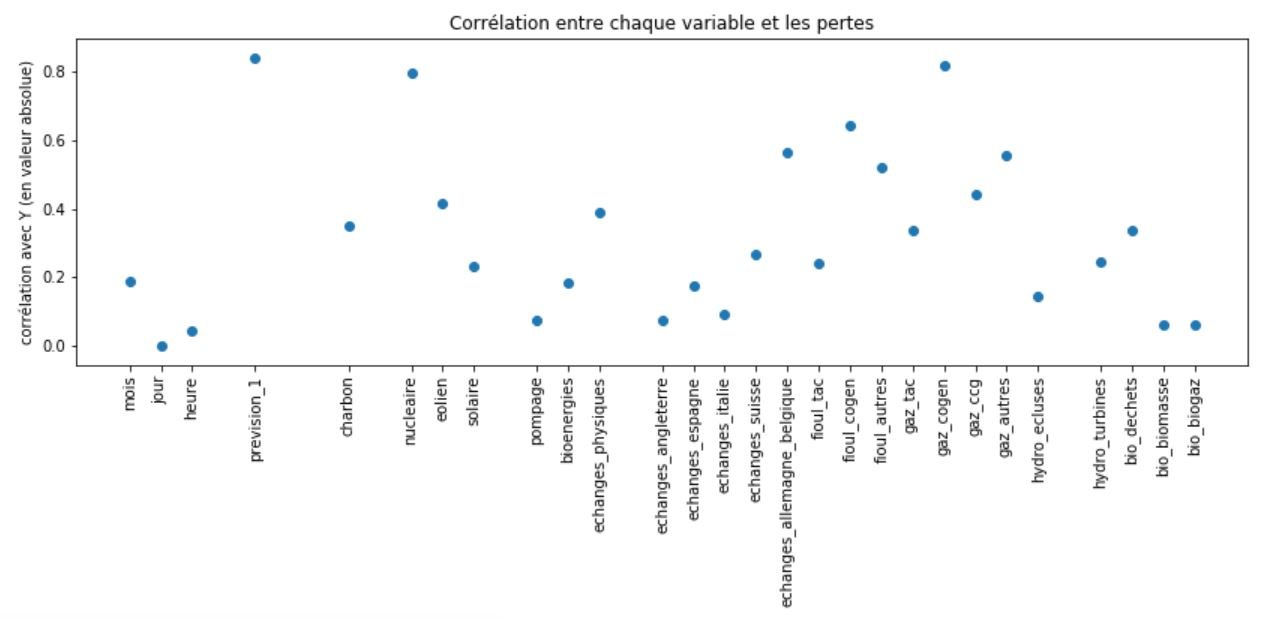
\includegraphics[scale=.5]{figures/pearson_y.JPG} Beaucoup de variables
peu significatives (\(\rho \approx \pm 0.5\))
\end{frame}

\begin{frame}[fragile]{P-value}
\protect\hypertarget{p-value}{}
p-valeur avec \texttt{scipy.stats} : probabilité du même \(\rho\) dans
un système décorrélé 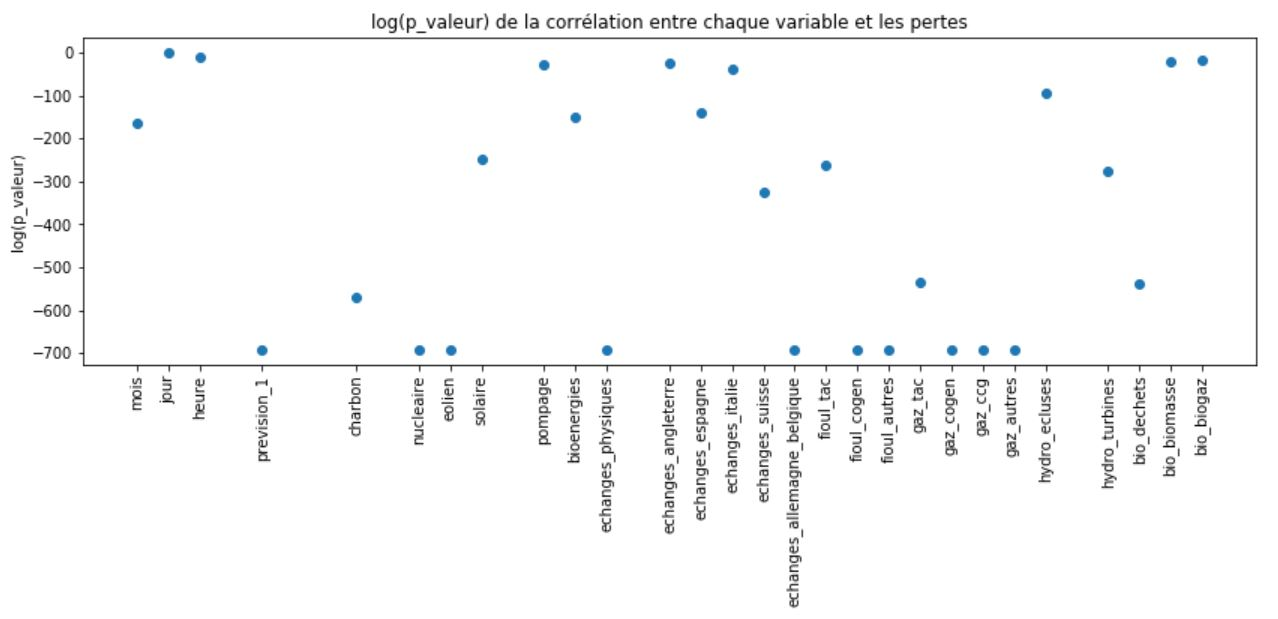
\includegraphics[scale=.5]{figures/log_p_value.JPG}
\end{frame}

\begin{frame}{P-value}
\protect\hypertarget{p-value-1}{}
Sans le log on trouve un intrus :
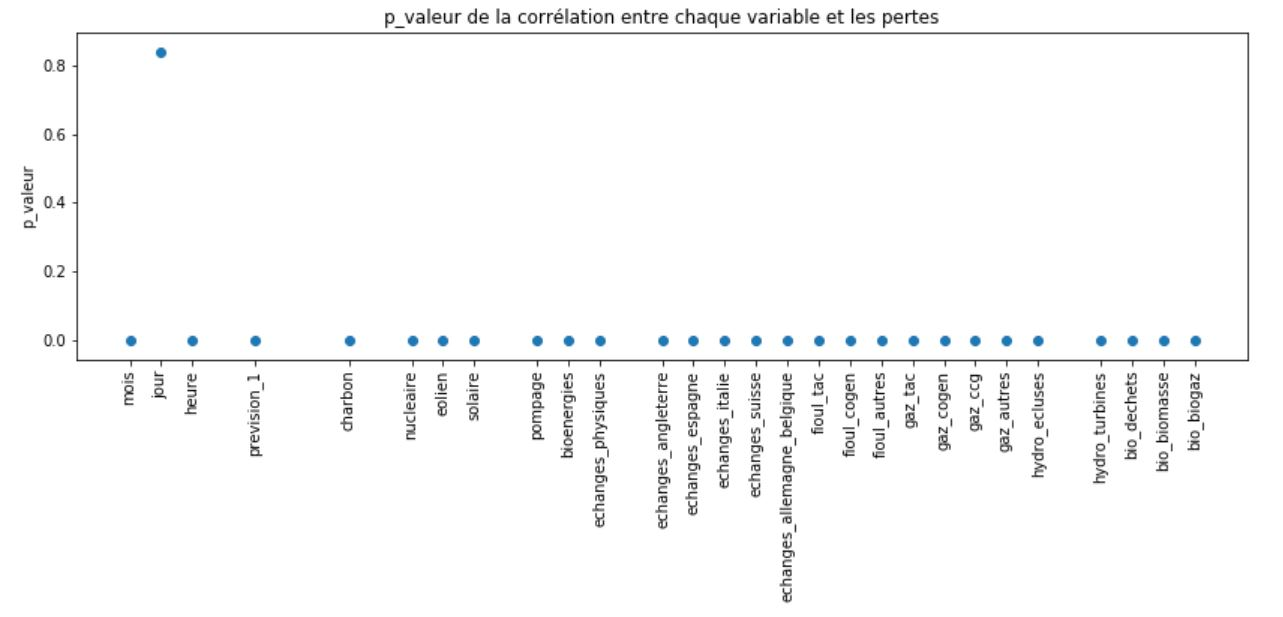
\includegraphics[scale=.5]{figures/p_value.JPG} En effet, peu de
variations périodiques significatives à l'échelle d'un mois
\end{frame}

\begin{frame}[fragile]{Corrélation avec les pertes}
\protect\hypertarget{corruxe9lation-avec-les-pertes-1}{}
\texttt{prevision\_1}, \texttt{nucleaire} et \texttt{gaz\_cogen}

\begin{itemize}
\tightlist
\item
  \(\rho\approx 0.8\) : forte corrélation
\item
  \texttt{nucleaire} et \texttt{gaz\_cogen} très corrélées : on peut
  n'en garder qu'une
\item
  p-value très basse
\end{itemize}
\end{frame}

\begin{frame}[fragile]{Corrélation avec les pertes}
\protect\hypertarget{corruxe9lation-avec-les-pertes-2}{}
\texttt{mois}, \texttt{jour}, \texttt{solaire} ainsi que des données
\texttt{bio} spécifiques (7 featues) :

\begin{itemize}
\tightlist
\item
  Corrélation à 0
\item
  Pas de relation linéaire : exclues pour la régression linéaire
\item
  En les excluant : \(R^2\) de 03805 à 0.799, soit 0.7\%
\item
  Comparé au doublons : 2 fois moins de perte, même nombre d'éliminés
\item
  On élimine aussi les fortes p-values (probablement décorrélées)
\end{itemize}
\end{frame}

\begin{frame}{Analyse en composantes principales}
\protect\hypertarget{analyse-en-composantes-principales}{}
Variables \(x_i\), covariance \(K\), composantes orthogonales \(c\) et
valeurs propres \(\lambda\) associées aux vecteurs \(e\). Corrélation
entre variable et composante principale :

\begin{equation}
\text{Corr}(c^l, x^j) = \frac{\sqrt{\lambda_l}e_l^j}{K_{ij}}
\end{equation}
\end{frame}

\begin{frame}{PCA}
\protect\hypertarget{pca}{}
On observe ces corrélations avec 5 puis 15 composantes principales, en
prenant le maximum pour chaque variable :
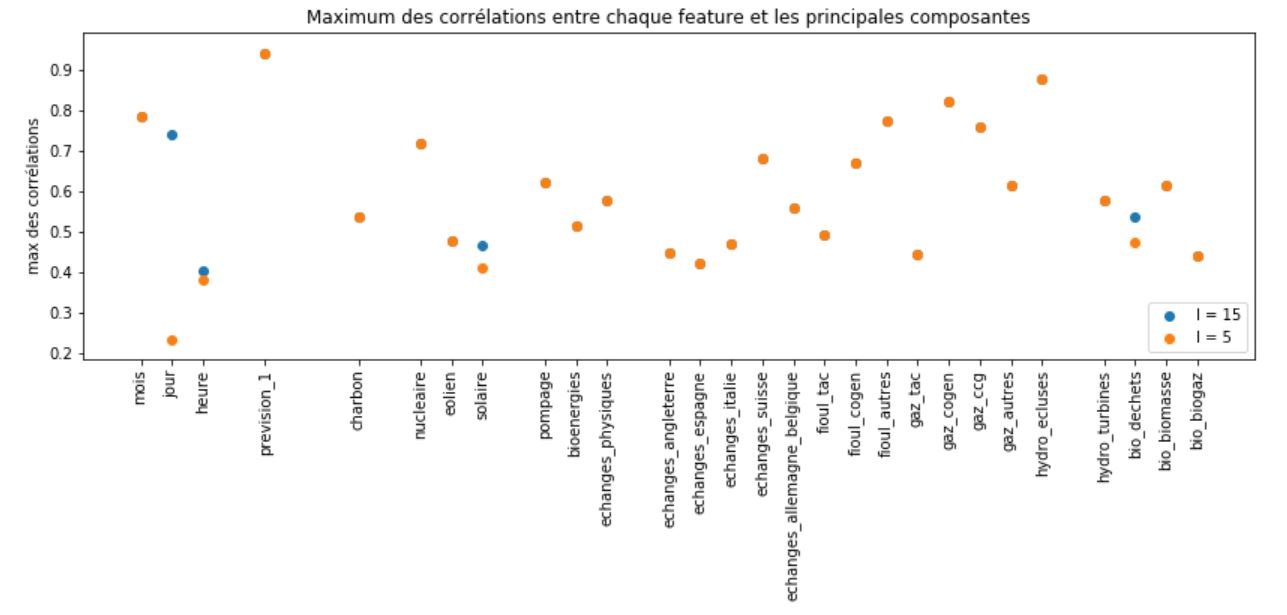
\includegraphics[scale=.5]{figures/max_pca.JPG}
\end{frame}

\begin{frame}{PCA}
\protect\hypertarget{pca-1}{}
Puis la somme des corrélations par variable :
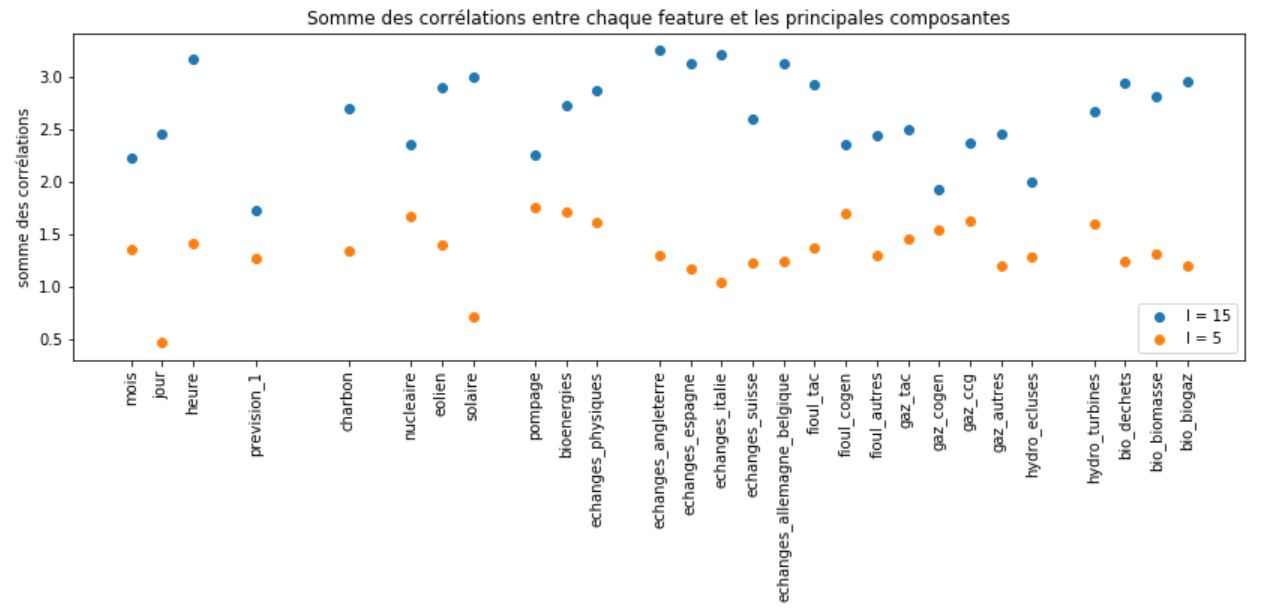
\includegraphics[scale=.5]{figures/sum_pca.JPG}
\end{frame}

\begin{frame}[fragile]{PCA}
\protect\hypertarget{pca-2}{}
\begin{itemize}
\tightlist
\item
  La consommation a un maximum très élevé pour une somme faible : elle
  est presque à elle seule une composante principale
\item
  \texttt{heure} \texttt{hydro\_ecluses} et \texttt{solaire} sont
  réparties sur plusieurs composantes
\item
  \texttt{heure} \texttt{solaire} et \texttt{echanges\_*} disparaissent
  en restreignant le nombre de composantes.
\end{itemize}
\end{frame}

\begin{frame}{k Nearest Neighbors}
\protect\hypertarget{k-nearest-neighbors}{}
On lance k-NN avec k=1, 5 puis 10, en mesurant le conjugué de l'erreur
relative. 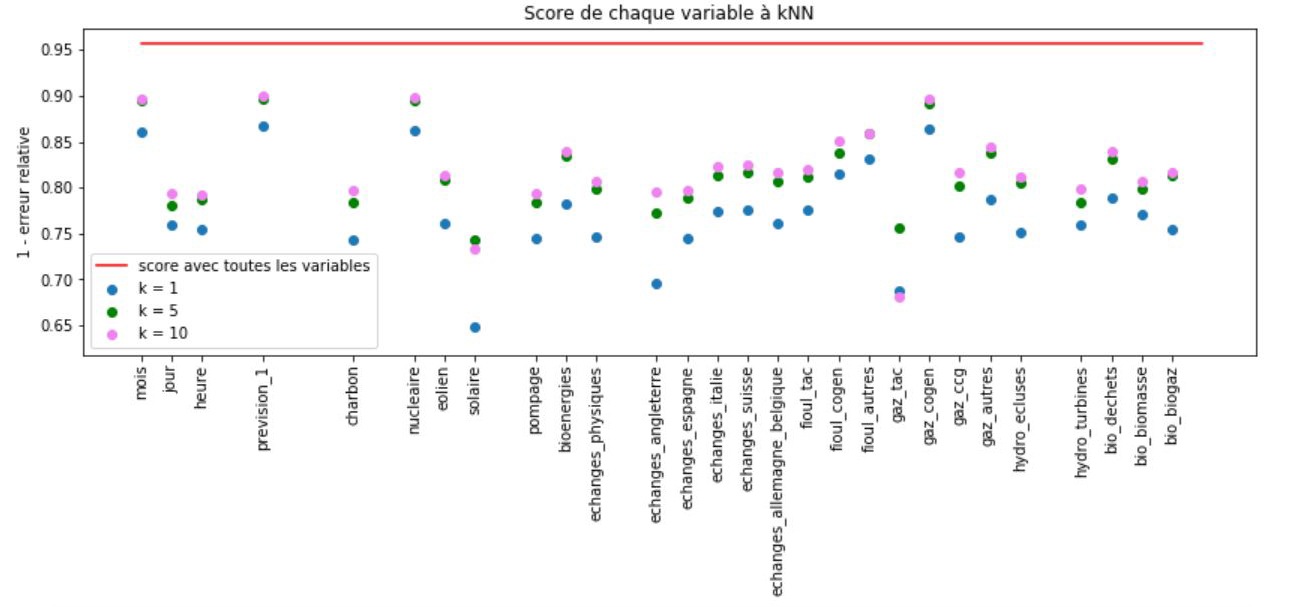
\includegraphics[scale=.5]{figures/knn.JPG}
\end{frame}

\begin{frame}[fragile]{k-NN}
\protect\hypertarget{k-nn}{}
\begin{itemize}
\tightlist
\item
  \texttt{mois}, \texttt{prevision\_1}, \texttt{nucléaire} et
  \texttt{gaz\_cogen} sont performantes, même avec peu de voisins
\item
  \texttt{solaire} et \texttt{gaz\_tac} sont peu performantes
\item
  Les autres dans une bande moyennée entre 0.75 et 0.9 : non concluant
\end{itemize}
\end{frame}

\begin{frame}{Support Vector Regressor}
\protect\hypertarget{support-vector-regressor}{}
Noyau gaussien de paramètre 0.001 et constante de tradeoff 1, entraîné
sur 10 époques et 100 observations.
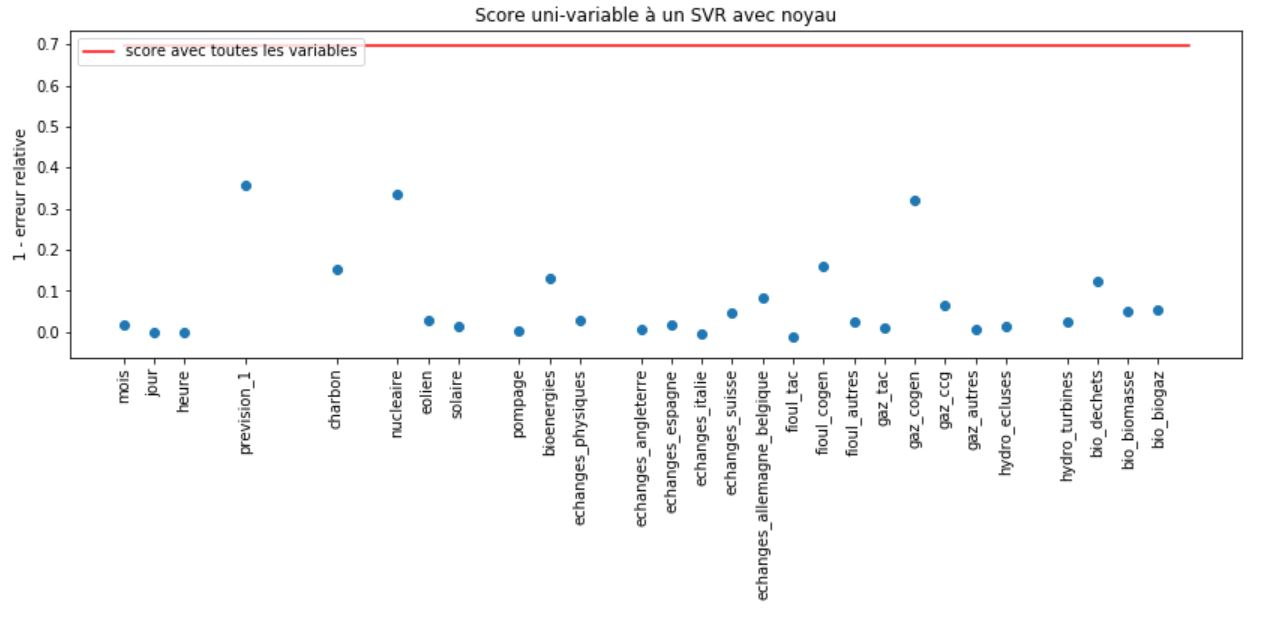
\includegraphics[scale=.5]{figures/svr.JPG}
\end{frame}

\begin{frame}[fragile]{SVR}
\protect\hypertarget{svr}{}
\begin{itemize}
\tightlist
\item
  On retrouve \texttt{prevision\_1}, \texttt{nucleaire} et
  \texttt{gaz\_cogen} performants
\item
  Quelques \(R^2\) négatifs : susceptibles de fausser les prédictions
\end{itemize}
\end{frame}

\begin{frame}{Poids de la régression linéaire}
\protect\hypertarget{poids-de-la-ruxe9gression-linuxe9aire}{}
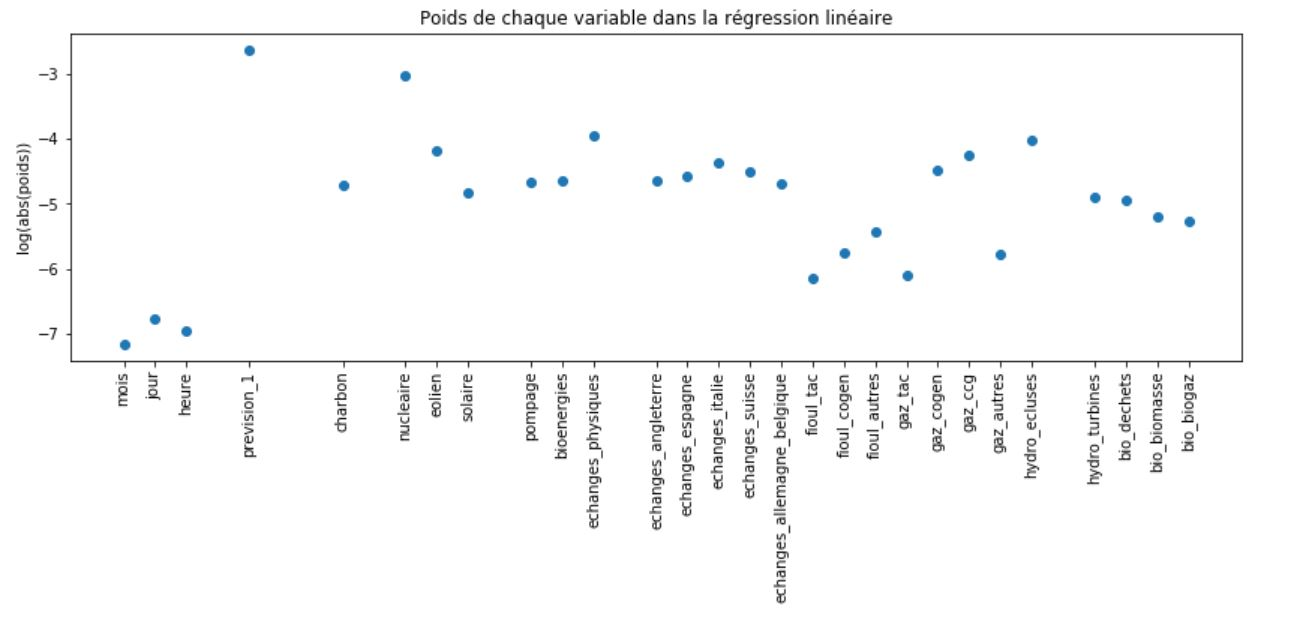
\includegraphics[scale=.5]{figures/poids.JPG} Les différences de poids
peuvent être dues aux différences d'échelle
\end{frame}

\begin{frame}{Test de student sur les poids}
\protect\hypertarget{test-de-student-sur-les-poids}{}
\begin{itemize}
\tightlist
\item
  Hypothèse nulle pour chaque poids : il est nul (donc variable inutile)
\item
  Test à 5\% : élimination de la moitié des variables (sans compter les
  doublons qui restent à éliminer)
\end{itemize}
\end{frame}

\hypertarget{conclusion}{%
\section{Conclusion}\label{conclusion}}

\begin{frame}{Difficultés}
\protect\hypertarget{difficultuxe9s}{}
\begin{itemize}
\tightlist
\item
  différentes installation python : contournement avec jupyter notebook,
  organisation du code
\item
  factorisation difficile : beaucoup de paramètres entrent en jeu
\item
  travail à distance
\end{itemize}
\end{frame}

\begin{frame}{Résultats}
\protect\hypertarget{ruxe9sultats}{}
\begin{itemize}
\tightlist
\item
  Élimination de nombreuses variables inutiles ou redondantes, en lien
  avec intuitions
\item
  Résultats très satisfaisants avec certains modèles
\end{itemize}

\begin{longtable}[]{@{}ll@{}}
\toprule
\emph{Variables conservées} & \emph{\(R^2\) de la prédiction
obtenue}\tabularnewline
\midrule
\endhead
Toutes & 0.865\tabularnewline
Test de Student & 0.858\tabularnewline
Test de Student inverse & 0.501\tabularnewline
Doublons & 0.849\tabularnewline
Toutes méthodes considérées & 0.833\tabularnewline
\bottomrule
\end{longtable}
\end{frame}

\begin{frame}{Pour aller plus loin}
\protect\hypertarget{pour-aller-plus-loin}{}
\begin{itemize}
\tightlist
\item
  Évolution de la relation entre variables explicatives potentielles et
  pertes
\item
  Transformation préalable des variables (périodicité notamment)
\end{itemize}
\end{frame}

\begin{frame}{Remerciements}
\protect\hypertarget{remerciements}{}
\begin{itemize}
\tightlist
\item
  Aboubakr MACHRAFI (stagiaire RTE)
\item
  Valentin CADORET, Virginie DORDONNAT (RTE)
\item
  Gabriel STOLTZ (ENPC)
\item
  David PICARD (ENPC)
\end{itemize}
\end{frame}
